\chapter{Testing (1000)}
\section{Functional Testing}
\begin{itemize}
	\item Method used
	\item Results
	\item Summary
\end{itemize}
\subsection{System Output}
show various playlists using different criteria
\section{Automated Testing}
\begin{itemize}
	\item Method used
	\item Results
	\item Summary
\end{itemize}
\begin{figure}[hp]
	\caption{PPOOOPOPO}
	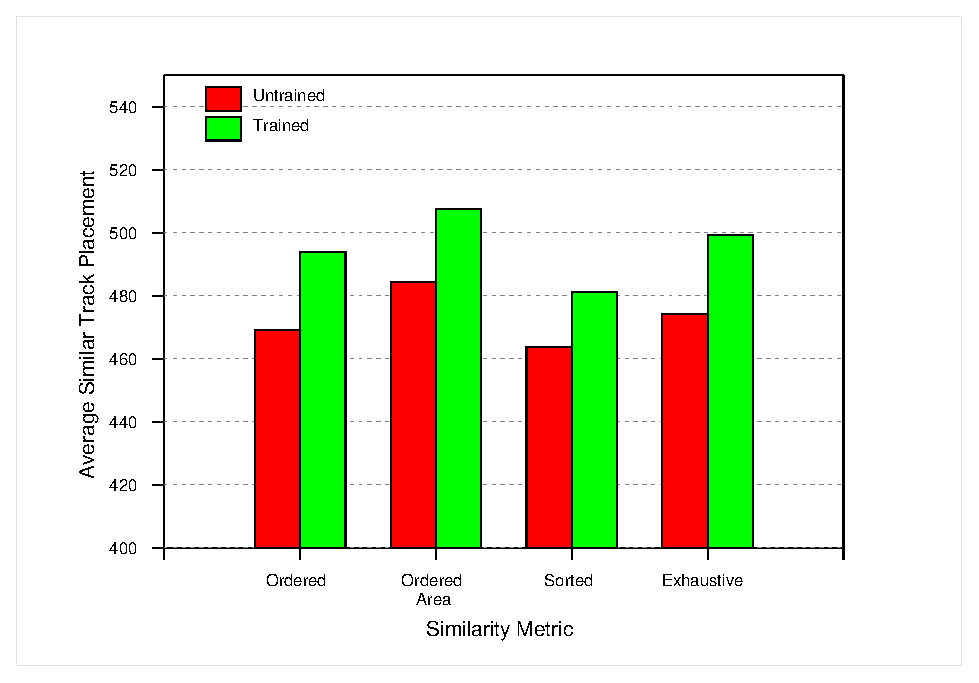
\includegraphics[width=\textwidth]{testing/graphs/comparison-metric-trained-untrained}
	\label{graph:trained-untrained}
\end{figure}
\section{User Testing(?)}
Do I even need to do this any more?
\begin{itemize}
	\item Method used
	\item Results
	\item Summary
\end{itemize}
